\chapter{Quantum platforms from semiconductors}

The interaction between structure and characteristics of matter is the foundation of material science. The applications of material science are unlimited, and if the reader takes a quick look around, hen will observe that every artifical material is made for a purpose, either being a bottle of water or a chair to sit in.

This chapter will serve as an introduction to material science from a practical point of view, with a special emphasis on solid-state semiconductors.


\section{Quantum technologies}

In this section we will give a brief overview of the current domain in quantum technological advances. This will not only give us insights in how the technology is being used today, but also grant us the opportunity to discuss key concepts that are fundamental to understand for this thesis. Importantly, it will motivate the reasoning for finding new materials that can be used in devices for this purpose.

\textit{Quantum technology} (QT) refers to practical applications and devices that utilise the principles of quantum physics as a foundation. Technologies in this specter are based on concepts such as \textit{superposition}, \textit{entanglement} and \textit{coherence}.

A quantum superposition refers to any two or more quantum states can be added together into another valid quantum state, such that every quantum state can be represented as a sum, or a superposition, of two or more distinct state. This is according to the wave-particle duality which phrase that every particle or another quantum entity may be described as either a particle or a wave. When measuring a superposition, however, the system falls back to one of the basis states that formed the superposition, destroying the original configuration.

A quantum entanglement refers to when a two- or many-particle state cannot be expressed independently of the state of the other particles, even when the particles are separated by a significant distance. As a result, the many-particle state is termed an entangled state \cite{Griffiths2017}.

Quantum coherence arise if two waves coherently interfere with each other and generate a superposition of the two states. Likewise, loss of coherence is known as \textit{decoherence}.

The terms superposition, entanglement and coherence are closely related. The two latter terms are the primary features of quantum mechanics that are lacking in classical mechanics, giving rise to paradoxes such as Einstein's famous Schrödingers cat, which is both dead and alive at the same time when in its coherent state inside a closed box.

Additionally, another concept that the reader should be familiar with is the famous Heisenberg uncertainty principle. It states that
\begin{align}
    \sigma_x \sigma_p \leq \frac{\hslash}{2},
    \label{eq:uncertainty}
\end{align}
where $\sigma_x$ is the standard deviation for the position and $\sigma_p$ is the standard deviation in momentum. This means that we cannot accurately predict both the position and momentum of the same particle at the same time. Thus, we often calculate the probability for a particle to be in a state which results in imaginable concepts such as an electron sky surrounding a neutron. However, it is often forgotten that equation \ref{eq:uncertainty} is an inequality, which means that it is possible to create a state where both the position and momentum is not-well defined, opposed to having both well defined.

\subsection{Quantum communication}

Quantum communication refers to the transfer of a state of one atom to another. This can be done with the use of a photon carrying a quantum state, which is termed a \textit{flying qubit}. A significant portion of quantum communication is also part of other quantum information theories such as quantum cryptography, which comes as a remedy to a rising paranoia concerning security \cite{Griffiths2002, Pavicic2006}.

%Classical cryptography encrypts information with the use of a key.

It is difficult to avoid someone eavesdropping a conversation, however, the problem fades away if the eavesdropper does not speak the language, which keeps the content of the conversation safe. Herein, we will refer to the conversation as a public key, and the content of the conversation as a private key. Albeit, we live in a digital world where most of our actions are increasingly being stored as information, and we could imagine that the eavesdropper in the latter example stored the conversation. Even if the content of the conversation was encrypted with a private key, it still presents a challenge, since encrypted information stored today could be deciphered in ten or twenty years' time\footnote{As an example, in Martin Gardner's \textit{Scientific American} column in $1976$ \cite{Taubes1994}, the $129$-digit RSA key was thought to be safe for $5000$ mips (million instructions per second) years, equal to $4 \times 10^{25}$ years. Only $17$ years later, the factorization was a reality and the public key was revealed to be ``The Magic Words are Squeamish Ossifrage'' \cite{Atkins1995}. To compare to todays fastest supercomputer Fugaku \cite{Top500} by making two \textit{very} rough estimations that flops and mips are approximately the same in addition to solely basing the calculation on computing power, the $129$-digit RSA private key would be found in less than half a second using Fugaku.}. In addition, the digital worlds encryption keys could be broken anytime by an imaginable complex algorithm, which could result in Armageddon. Consequently, finding an encryption method that could make information either impossible to eavesdrop or make the security unbreakable forever is very desirable. This is the ultimate goal of quantum cryptography \cite{Pavicic2006}.

\begin{wrapfigure}{r}{0.5\textwidth}
  \centering
  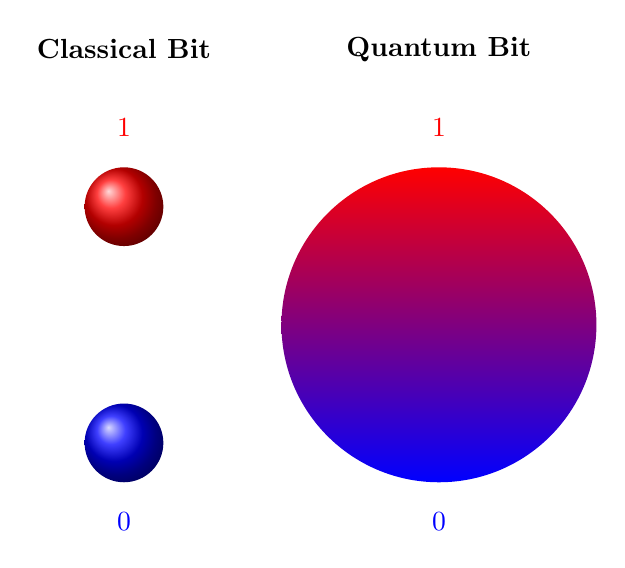
\begin{tikzpicture}[scale=1]
    \node[font=\bfseries] at (0,2) {Classical Bit};
    \node[font=\bfseries] at (4,2) {Quantum Bit};

    \node[color=red] at (0,1) {$1$};
    \node[color=blue] at (0,-4) {$0$};

    \node[shade,shading=ball,circle,ball color=blue,minimum size=1cm] (ball) at (0,-3) {};
    \node[shade,shading=ball,circle,ball color=red,minimum size=1cm] (ball) at (0,0) {};

    \node[color=red] at (4,1) {$1$};
    \node[color=blue] at (4,-4) {$0$};
    \node[shade, shading=ball,circle,top color=red, bottom color=blue, minimum size=4cm] (ball) at (4,-1.5) {};
  \end{tikzpicture}
  \caption{Conceptual illustration of the two-level classical bit, which are restricted to the boolean states 1 (true) or 0 (false), and the quantum bit that can be in any superposition of the states 0 or 1.}
  \label{fig:qubit and bit}
\end{wrapfigure}
The idea is to pass information in the form of a quantum bit, or \textit{qubits} for short. They are the building blocks of quantum computers, and as opposed to a conventional 0- or 1-bits that classical computers are based on, they can inhabit any superposition of the states 0 or 1. This approach is termed the \textit{quantum key distribution} (QKD) \cite{Gisin2002, Gisin2007}. Now, if a wild eavesdropper would try to measure the information, the nature of quantum physics tells us that the original configuration would be destroyed and the receiver would be alerted of the eavesdropper. Furthermore, if the eavesdropper would try to make a copy of the message, the copying itself would be limited of the no-cloning theorem \cite{Gisin2002} which declare that quantum states cannot be copied.

A clever approach to ensure confidentiality is to send the encryption key of the information before sending the actual encrypted information. If the key is received unperturbed then no one knows the key and it can be safely used. If it turns out perturbed, confidentiality is still intact since the key does not contain any information and can be discarded \cite{Gisin2002}. It should be noted that this requires both the sender and receiver to not only have each their quantum computer to store qubits in its memory, but also that they will need to initially exchange a common secret which is later expanded, making quantum key \textit{expansion} a more exact term for QKD \cite{Pavicic2006, Gisin2007}.

Most applications and experiments use optical fibers for sending information via photons, with the distance regarded as the main limitation. This is reasoned by that classical repeaters are unable to enhance quantum information because of the no-cloning theorem, making photon loss in optical fiber cables inevitable. Thus, quantum communication must reinvent the repeater concept, using hardware that preserves the quantum nature \cite{Acin2018}. Nonetheless, secure QKD up to 400km has recently been demonstrated using optical fibres in academic prototypes \cite{Boaron2018}.

\subsection{Quantum sensing}

Measurements are part of our digital world today to a great extent. There would be no way to exchange goods, services or information without some extent of reliable and precise measurements \cite{Acin2018}. Thus, improving the accuracy of sensors for every measurement done is desirable. One method to improve measurements can be by utilising quantum sensors, which is the use of a quantum property, such as a quantum object or quantum coherence, to measure a physical quantity \cite{Degen2017}. This is possible because quantum systems are easily receptive to pertubations of its surroundings due to decoherence, and can be used to detect physical properties such as time, rotations, temperature and pressure \cite{Degen2017}.

For a quantum system to be able to function as a quantum sensors, a few of the criterias formulated by DiVincenzo has to be met \cite{DiVincenzo2000}. Firstly, the quantum system needs to have discrete and resolvable energy levels. The quantum system also needs to be controllably initialised into a state that can be identified and coherently manipulated by time-dependent fields. Lastly, the quantum system needs to be able to interact with the physical property one wants to measure through a coupling parameter \cite{Degen2017}.

It is also possible to also exploit quantum entanglement to improve the precision of a measurement. This gain of precision is used to reach what is called the Heisenberg-limit, which states that the precision scales as the number of particles $N$ in an idealized quantum system \cite{Degen2017, Acin2018}, while the best classical sensors scale with $\sqrt{N}$.

\subsection{Quantum computation}
%The evolution of the digital worlds computational powers is a remarkable piece of history
The start of the digital world's computational powers can be credited to Alan Turing. In 1937, Turing \cite{Turing1937} published a paper where he described the \textit{Turing machine}, which is regarded as the foundation of computation and computer science. It states that only the simplest form of calculus, such as boolean Algebra ($1$ for true and $0$ for false), is actually computable. This required developing hardware that could handle classical logic operations, and was the basis of transistors that are either in the state ON or OFF depending on the electrical signal. Equipped with a circuit consisting of wires and transistors, commonly known as a computer, we could develop software to solve all kinds of possible applications.

Driven by the development of software, conventional computers has, in accordance to Moore's law \cite{Moore1965}, doubled the amount of transistors on integrated circuit chips every two years as a result of smaller transistors. Furthermore, the clock frequency has enhanced with time, resulting in doubling of computer performance every 18 months \cite{Pavicic2006}. Alas, miniaturization cannot go on forever as transistors are mass-produced at $5$nm today and are expected to reach a critical limit of $3$nm in the following years \cite{Gwennap2020}.

To sustain the digital worlds increasing computational demand, other alternatives than the conventional classical computer must be explored. This is where quantum computation comes into the picture. A qubit has a quantum nature that brings it to the center of attention in a quantum computation\footnote{There exists other systems such as the quantum d-state system, known as \textit{qudits}, that can also be utilised in quantum computation \cite{Ladd2010}.}. The most promising implementations of qubits are the polarization of photons, the spin of atoms, nuclei or quantum dots, currents running through superconducting Josephson junctions and the spin or charge of electrons \cite{Bathen2020}. The reader is encouraged to read a more thorough review of qubit-implementations in reference \cite{Acin2018}.

The architecture of a quantum computer is dependent on a set of quantum logic gates that perform unitary transformations on sets of qubits \cite{DiVincenzo2000, Ladd2010}. Other implementations of quantum computers exists, such as the adiabatic quantum computer. This approach is not based on gates, but on defining the answer of a problem as the ground state of a complex network of interactions between qubits, and then controlling the interactions to adiabatically evolve to the ground state \cite{Mizel2007}.

It has been demonstrated that exponentially complex problems can be reduced to polynomially complex problems for quantum computers \cite{Pavicic2006}. For example, a quantum search algorithm found by Grover \cite{Grover1997} offers a quadratic speed-up compared to classical algorithms, which initally is not a huge speed-up but indeed has a limitless spectrum of applications. Additionally, Shor's quantum integer factorization algorithm \cite{Shor1994} present an exponential speed-up, and can be used to break the widely used RSA-scheme in cryptography. Even more impressively, Google reported in $2019$ that they ran a random number generator algorithm using 53 qubits on a superconducting processor in $200$ seconds which would take $10.000$ years for a classical computer \cite{Martinis2019}. It is expected that quantum computers will excel in exceedingly complex problems, while many simpler tasks may not see any speed-up at all. Hence, it is not expected that quantum computers will run classical computers out of business, but rather that they will coexist for each their purpose. However, it is not to avoid that both quantum  hardware and -software is in its preliminary phase of development, and it will be interesting to follow up the progression the following years.

Quantum computing is a highly sought-after goal, but there are extensive challenges that needs to be adressed. Controlling a complex many-qubit system is difficult, since it is not always possible to establish interactions between qubits \cite{DiVincenzo2000}. Additionally, decoherence and other quantum noise occurs as a result to the high volatility of quantum states, making quantum state manipulation prone to errors. The \textit{quantum error correction} protocols and the theory of \textit{threshold theorem} deals with this vulnerability, stating that noise most likely does not pose any fundamental barrier to the performance of large-scale computations \cite{Pavicic2006}.



\section{Crystal structure}


Solid materials are formed by densely packed atoms. These atoms can randomly occur through the material without any long-range order, which would categorize the material as an \textit{amorphous solid}. Amorphous solids are frequently used in gels, glass and polymers \cite{BenStreetman2015}.

However, the atoms can also be periodically ordered in small regions of the material, classifying the material as a \textit{polycrystalline solid}. All ceramics are polycrystalline with a broad specter of applications ranging from kitchen-porcelain to orthopedical bio-implants \cite{Renganathan2018}.

\begin{figure}
  \centering
\begin{subfigure}{.5\linewidth}
\centering
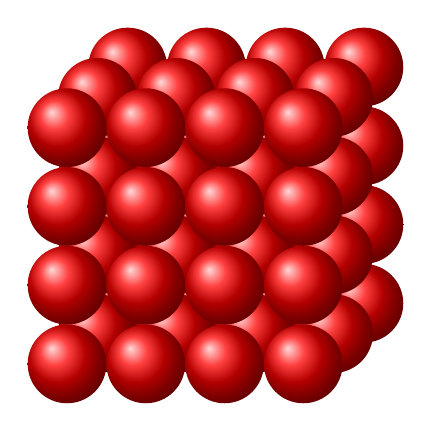
\begin{tikzpicture}
  \foreach \z in {1,2,3}{
  \foreach \i in {3,2,1,0}{% This one doesn't matter
    \foreach \j in {3,2,1,0}{% This will crate a membrane
        \shade[ball color=red] ({\i},{\j},\z) circle(0.5);
      }
    }
  }
\end{tikzpicture}
\subcaption{} \label{fig:M1}
\end{subfigure}%
\par\bigskip

\begin{subfigure}{1.0\linewidth}
\centering
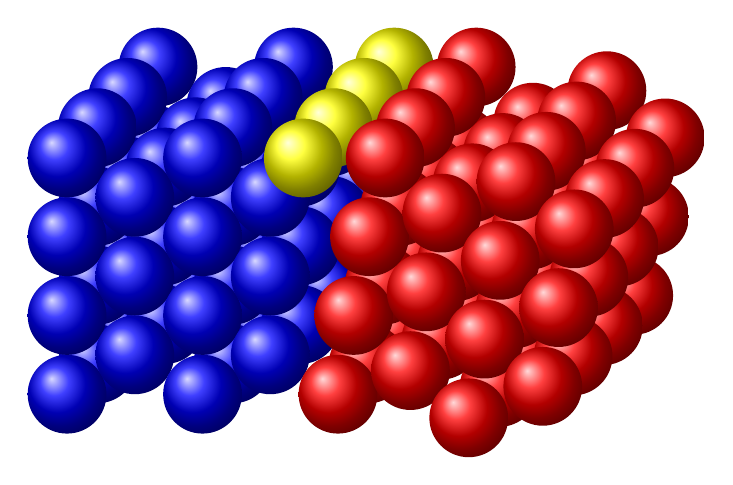
\begin{tikzpicture}
    \foreach \x in {0,1,2,3}{%
      \foreach \z in {0,1,2,3}{%
      \shade[ball color=blue] (0,\x,\z) circle(0.5);
      }
    }
    \foreach \x in {0.5,1.5,2.5}{%
      \foreach \z in {0,1,2,3}{%
      \shade[ball color=blue] ({1*sqrt(0.74)},\x,\z) circle(0.5);
      }
    }
    \foreach \x in {0,1,2,3}{%
      \foreach \z in {0,1,2,3}{%
      \shade[ball color=blue] ({2*sqrt(0.74)},\x,\z) circle(0.5);
      }
    }
    \foreach \x in {0.5,1.5,2.5}{%
      \foreach \z in {0,1,2,3}{%
      \shade[ball color=blue] ({3*sqrt(0.74)},\x,\z) circle(0.5);
      }
    }
    \foreach \z in {0,1,2,3}{%
      \shade[ball color=yellow] ({3},3,\z) circle(0.5);
    }
    \foreach \y in {0,1,2,3}{%
      \foreach \z in {0,1,2,3}{%
      \shade[ball color=red] ({4*sqrt(0.74)+0.2*\y},\y,\z) circle(0.5);
      }
    }
    \foreach \y in {0.3,1.3,2.3}{%
      \foreach \z in {0,1,2,3}{%
      \shade[ball color=red] ({5*sqrt(0.74)+0.2*\y},\y,\z) circle(0.5);
      }
    }
    \foreach \y in {-0.3,0.7,1.7,2.7}{%
      \foreach \z in {0,1,2,3}{%
      \shade[ball color=red] ({6*sqrt(0.74)+0.2*\y},\y,\z) circle(0.5);
      }
    }
    \foreach \y in {0.1,1.1,2.1}{%
      \foreach \z in {0,1,2,3}{%
      \shade[ball color=red] ({7*sqrt(0.74)+0.2*\y},\y,\z) circle(0.5);
      }
    }


\end{tikzpicture}
\subcaption{} \label{fig:M2}
\end{subfigure}%
\par\bigskip

\begin{subfigure}{1.0\linewidth}
\centering
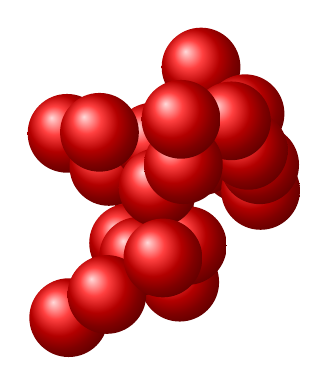
\begin{tikzpicture}
  \foreach \z in {0,...,24}{
    \shade[ball color=red] ({rand*1.5},{rand*1.5},{rand*1.5}) circle(0.5);
  }
\end{tikzpicture}
\subcaption{} \label{fig:M3}
\end{subfigure}
\par\bigskip
\caption{Different degrees of ordered structures, where (a) is a crystalline of a simple cubic lattice, (b) is a polycrystalline of a hexagonal lattice, and (c) is an amorphous. }
\label{fig:crystalstructure}
\end{figure}
A third option is to have these atoms arranged with infinite periodicity, making the material a \textit{crystalline solid} or more commonly named a \textit{crystal}. The three options are visualised in figure \ref{fig:crystalstructure}.

The periodicity in a crystal is defined in terms of a symmetric array of points in space called the \textit{lattice}, which can be simplified as either a one-dimensional array, a two-dimensional matrix or a three dimensional vector space, depending on the material. At each lattice point we can add an atom to make an arrangement called a \textit{basis}. The basis can be one atom or a cluster of atoms having the same spatial arrangement. For every crystal, there exists periodically repeated building blocks called \textit{cells} which represents the entire crystal. The smallest cell possible is called a \textit{primitive cell}, but such a cell only allows lattice points at its corners and it is often quite rigid to work with when the structure becomes complex. As a solution, we will consider the \textit{unit cell}, which allows lattice points on face centers and body centers. \footnote{Figur av enkleste gitter fcc, bcc og sc? tikz}

\section{The perovskite structure}

One known crystal structure is the perovskite structure. They have an $ABO_3$ stoichiometry whose symmetri belong to one of 15 space groups identified by Lufaso \& Woodward \cite{Lufaso2001}, such as the cubic, orthorombic and tetragonal, to name a few. The A atom is nine- to 12-fold coordinated by oxygen, while the B atom is sixfold coordinated by oxygen, and the $BO_6$ octahedra are connected to the corners in all three directions.

\begin{wrapfigure}{r}{0.5\textwidth}
  \centering
  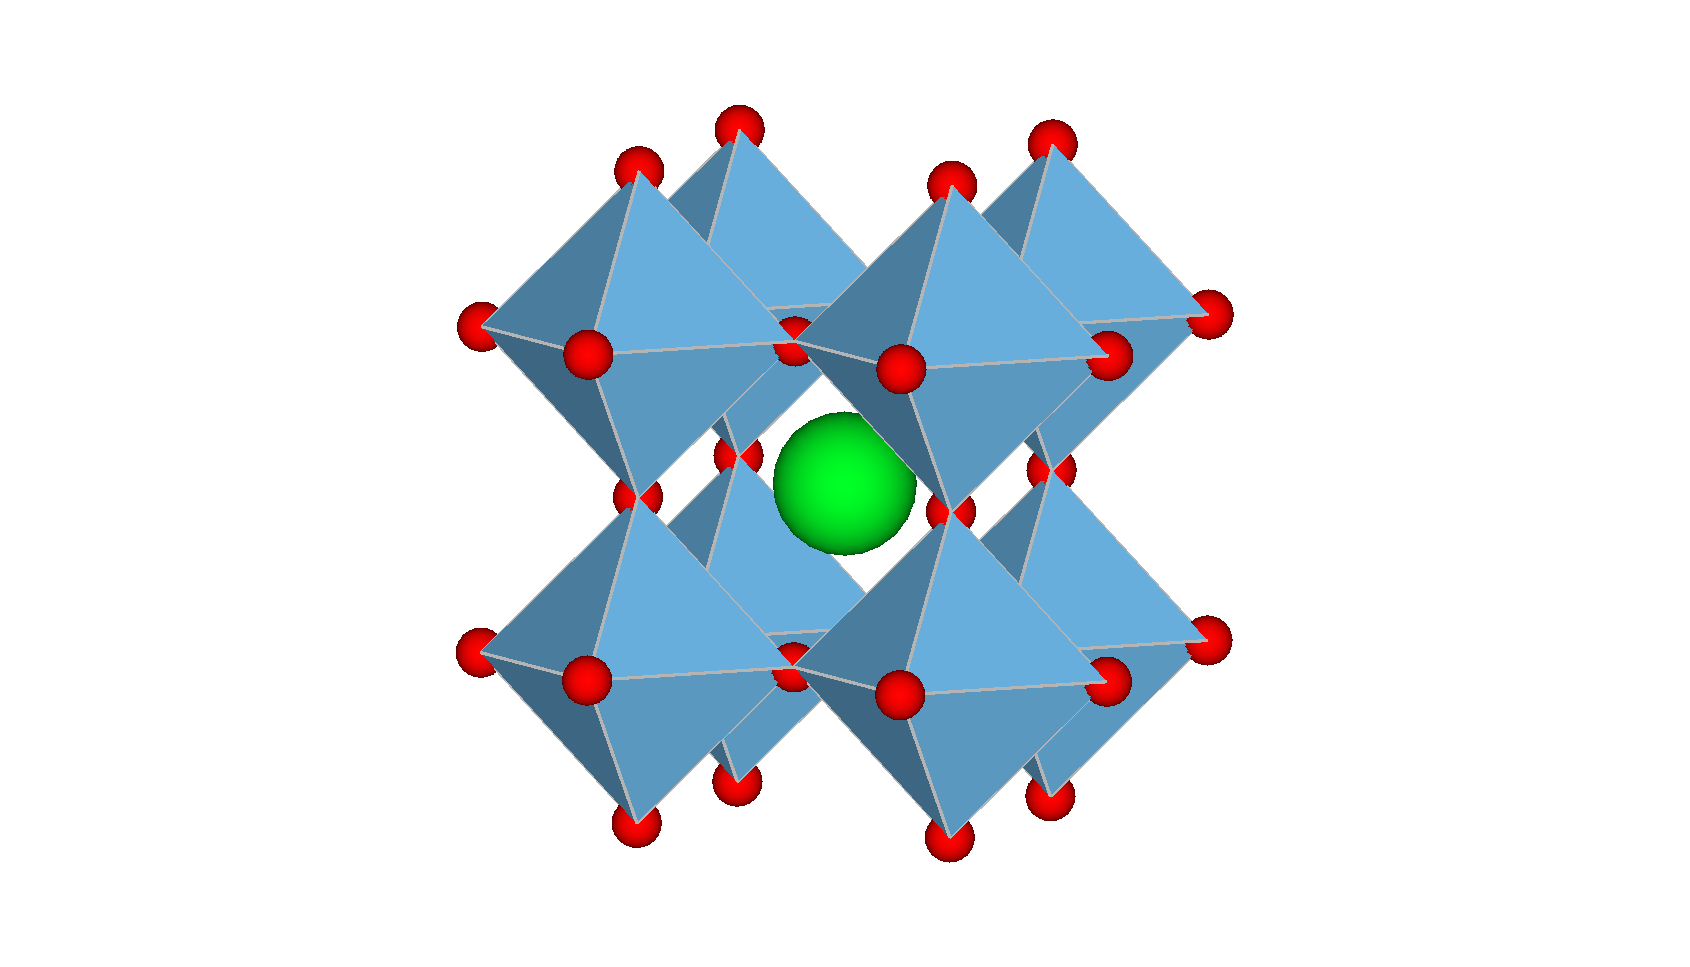
\includegraphics[width=0.48\textwidth]{theory/figures/SrTiO3_mp-5229_primitive.pdf}
  \caption{A crystal structure of SrTiO$_3$ which is a cubic perovskite. The red atoms are oxygen, whereas the green atom is strontium, and inside every corner-sharing BO$_6$ octahedral unit is a titanium atom.}
  \label{fig:pic}
\end{wrapfigure}

The motivation behind the research of perovskites is reasoned by that there are a large amount of possible ABO$_3$ chemistries, whereas a significant portion of these that takes the perovskite structure. They have a broad specter of applications, ranging from high-temperature superconductors \cite{Bednorz1988}, ionic conductors \cite{Boivin1998}, and  multiferroic materials \cite{Cheong2007}. Additionally, adding a perovskite structured compound to solar cells has reportedly resulted in higher performance efficiency while being cheap to produce and simple to manufacture \cite{IbnMohammed2017, Chen2014}, however, that includes the use of hybrid organic-inorganic compounds and excludes the use of oxygen.

\section{First principles of semiconductors}

Isolated atoms have distinct energy levels, where the Pauli exlusion principle \cite{Pauli1925} states for fermions that each energy level can accomodate two electrons of opposite spin. In a solid, the discrete energy levels of the isolated atom spread into continuous energy bands for the solid since the wavefunctions of the electrons in the neighboring atoms overlap \footnote{her er det mulighet for en kul figure fra diskret energi til continous band. Mena3000-boka}. Hence, an electron is not neccessarily localized at a particular atom anymore as it would for a system with an isolated atom. Every material has a unique band structure, similar to every human have their unique fingerprint.

\begin{wrapfigure}{r}{0.35\textwidth}
  \begin{minipage}{\linewidth}
    \centering\captionsetup[subfigure]{justification=centering}
  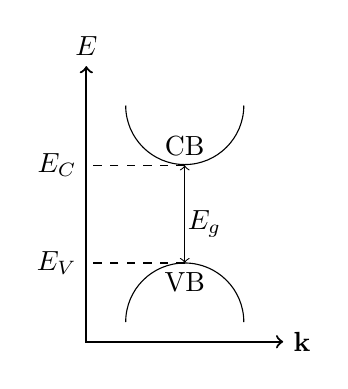
\begin{tikzpicture}[scale=1]
      \draw [<->,thick] (0,3.5) node (yaxis) [above] {$E$}
          |- (2.5,0) node (xaxis) [right] {$\textbf{k}$};
      \draw (0.5,0.25) arc(180:0:0.75cm);
      \draw (2.0,3.0) arc(0:-180:0.75cm);
      \coordinate (VB) at (1.25,1.0);
      \coordinate (CB) at (1.25,2.24);
      \draw[<->] (CB) node[above] {CB}
        -| (VB) node[below] {VB};
      \draw[dashed] (VB) -- (0,1.0) node[left]{$E_V$};
      \draw[dashed] (CB) -- (0,2.24) node[left]{$E_C$};
      \node at (1.5,1.5) {$E_g$};
  \end{tikzpicture}
  \subcaption{}
  \label{fig:directbandgap}
  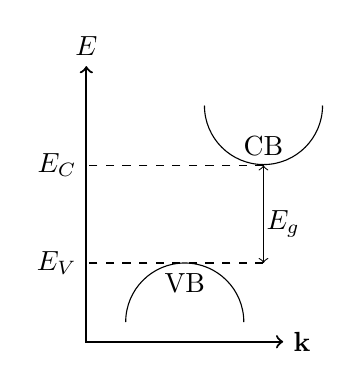
\begin{tikzpicture}[scale=1]
      \draw [<->,thick] (0,3.5) node (yaxis) [above] {$E$}
          |- (2.5,0) node (xaxis) [right] {$\textbf{k}$};
      \draw (0.5,0.25) arc(180:0:0.75cm);
      \draw (3.0,3.0) arc(0:-180:0.75cm);
      \coordinate (VB) at (2.25,1.0);
      \coordinate (CB) at (2.25,2.24);
      \draw[<->] (CB) node[above] {CB}
        -| (VB);
      \draw[dashed] (VB) -- (0,1.0) node[left]{$E_V$};
      \draw[dashed] (CB) -- (0,2.24) node[left]{$E_C$};
      \node at (2.5,1.5) {$E_g$};
      \node at (1.25,0.75) {VB};
  \end{tikzpicture}
  \label{fig:indirectbandgap}
  \subcaption{}
  \end{minipage}
  \caption{A schematic drawing of a (a) direct bandgap and an (b) indirect bandgap.}
\end{wrapfigure}

Which energy bands that are occupied by electrons, is the key in understanding the electrical properties of solids. The highest occupied electron band at $0$ K is called the valence band (VB), while the lowest unoccupied electon band is called the conduction band (CB). In between the two bands, we find an area that contains no electron energy states which is known as the band gap and its energy is denoted as $E_g$.

To be able to accelerate electrons in a solid using an electrical field, they must be able to move into new energy states. At $0$ K, the entire valence band of a semiconductor is full with electrons and no available new states, making it impossible to flow current through the material. This can be solved by using either thermal or optical energy to excite energies from the valence band to the conduction band, in order to \textit{conduct} electricity. In room temperature, many semiconductors will be able to have excited electrons in the conducting band solely from thermal energy matching the energy band gap \cite{BenStreetman2015}.

In some scenarios, thermal or optical energy is not sufficient for an excitation since the energy bands are also dependent by a crystal momentum. A difference in the momentum of the minimal-energy state in the conduction band and the maximum-energy state in the valence band, is known to be an \textit{indirect bandgap} as seen in figure \ref{fig:directbandgap}. If there is no difference at all, the material has a \textit{direct bandgap}, which is visualized in figure \ref{fig:indirectbandgap}.




%When isolated atoms are brought together to form a solid, various interactions occur between neighboring atoms. These interactions are the basis that forms the varied electrical properties of solids. . Each energy level

%The interactions between the electrons in a solid defines what kind of bonding there is, and can result in ionic bonding, metallic bonding or covalent bonding alone or mixed together.


 %A solid that conducts electrical current is, by definition, a metal. Every solid that has its own characteristic energy

 %On the other hand, a material that does not conduct electrical current is an insulator.

 \newpage
